\section{Ensemble}
A number of different strategies for combining the ensemble members will be described in this section. This includes averaging and weighted averaging the detections. The method for inferring each of the ensemble will be the same apart from the combination set. This is shown in \figref{ensemble_general}. Firstly, for a object proposal in an image found with the \gls{rpn} each network will infer a bounding box and associated confidence for all classes. After this the given ensemble combination method determines the final detection. 
\begin{figure}[H]
  \centering
    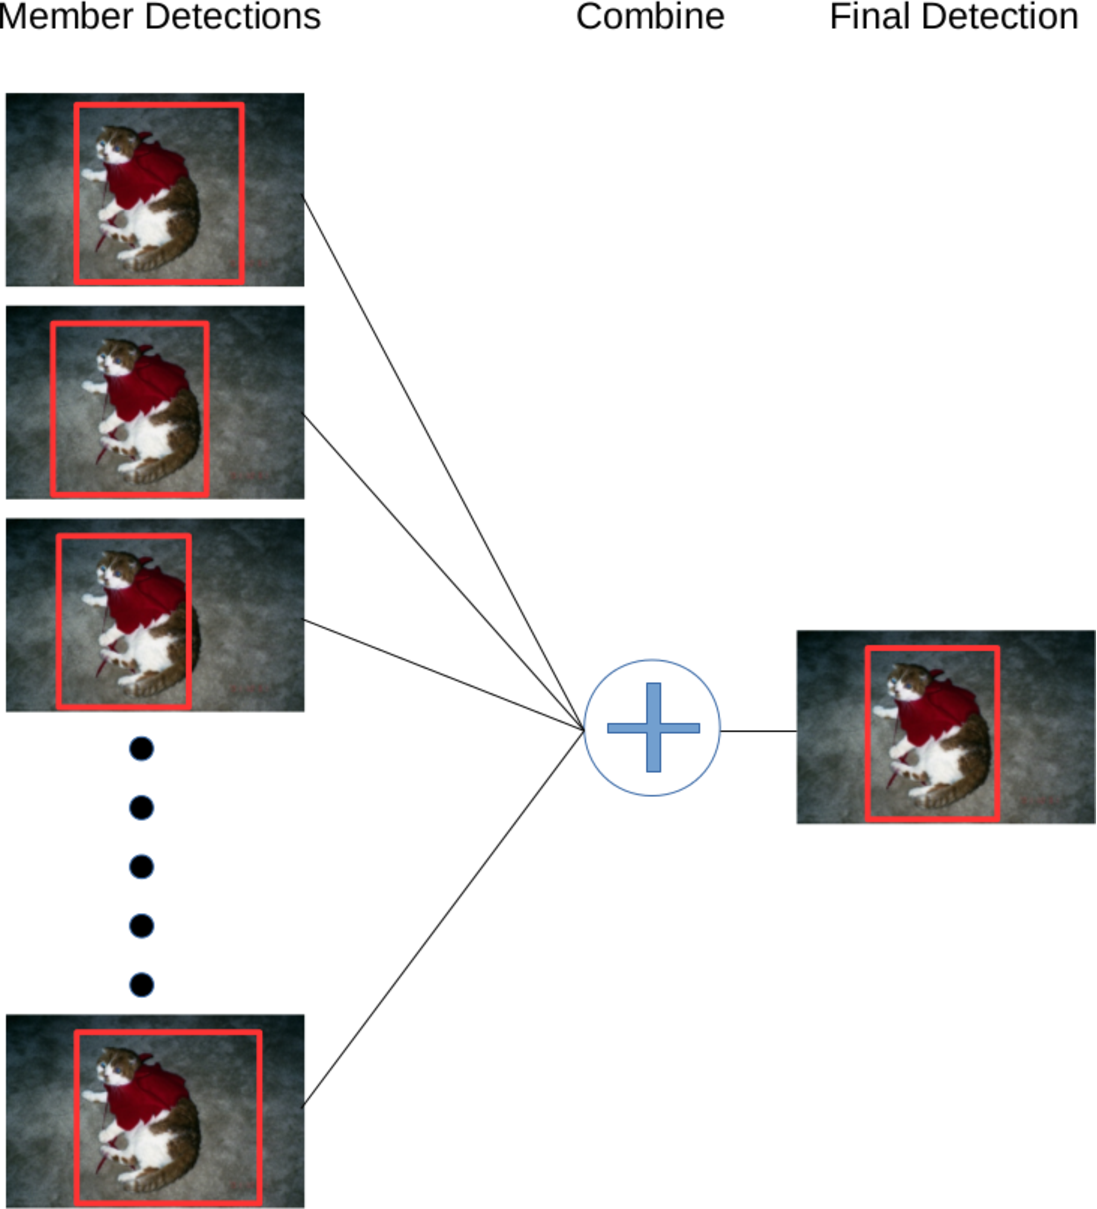
\includegraphics[width=0.5\textwidth]{Figs/Implementation/ensemble.pdf}
      \caption{}
    \label{fig:ensemble_general}
\end{figure}

A number of different combination strategies will be presented and evaluated in the remainder of this section. 

\subsection{Average Ensemble}
One of the combination strategies is similar to that used when evaluating the resolution-aware object detector in \sectionref{resawareSec}. Each of the five ensemble factors are weighted evenly in the overall ensemble. Within each ensemble factor pair, the detection for one of the pairs will be chosen and the other discarded. This is determined by where the given factor lies in relation to the training data distribution. For example, if for the given test image it is measured with Deep IQA to have JPEG compression below the threshold used to split the data, then the detection found using the model trained on that data will be used. This results in five detections that will be weighted equally to find the final detection by:

\begin{equation}
  E_{j} = \frac{1}{n} \sum_{i=1}^{n} p_{i,j} 
\end{equation}
where $n$ is the number of detections found by the $n$ ensemble factor, $p$ is the detection result to be averaged and $i$ represents one of the ensemble factors. Finally, $j$ is one of the five values found by each detection, namely the four corners of the bounding-box and the associated confidence.


\subsection{Weighted Average Ensemble}
Each of then 10 trained networks will be used on all object proposals found using the \gls{rpn}. Weights will be distributed evenly across each of the five different types of factors. The weighted average ensemble is determined for each bounding-box and the associated confidence by:

\begin{equation}
	E_{j} = \frac{1}{n} \sum_{i=1}^{n} w_ip_{i,j} 
\end{equation}

Weights are determined in pairs for each of the 5 ensemble factors, where the total sum of weights is equal to $n$. If each detection were to be weighted equally all $w$ would be equal to 1. As the weights are calculated in pairs each ensemble factor is overall weighted equally as the pair of weights can at most be equal to 2. By using this tactic in between the two sets of network for a given factor can be weighted differently but overall each factor is weighted equally.
Weights for a given factor is found according to where the the test image lies for that factors training distribution data. For example, the subsets of training data for Gaussian blur was determined according to the line shown in \figref{blur_dist}. 

\add[inline]{line showing split in training data}

\begin{figure}[H]
  \centering
    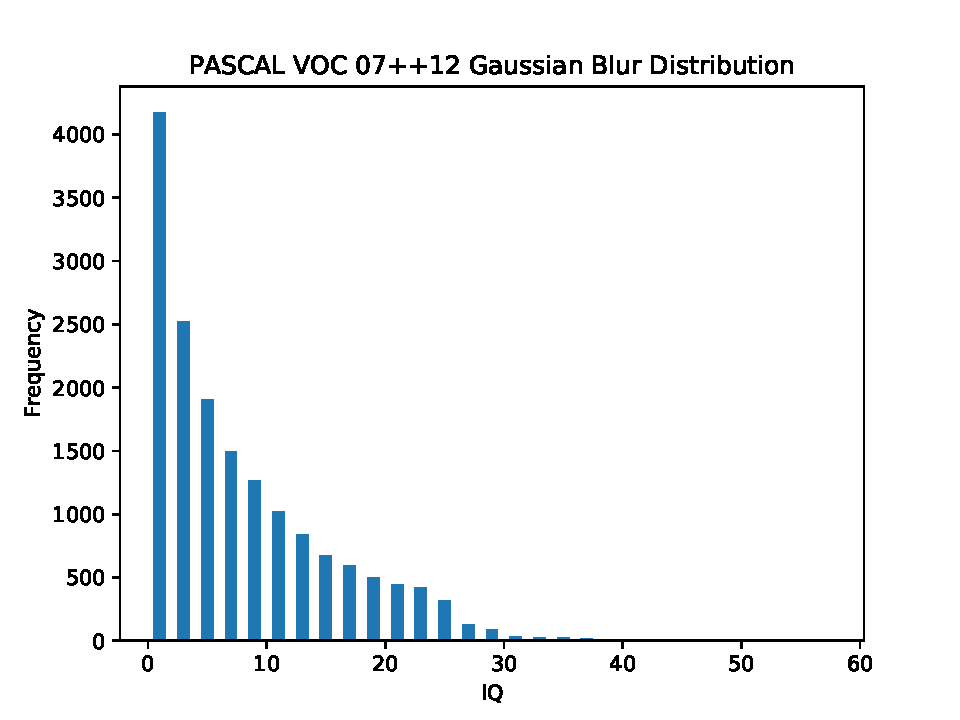
\includegraphics[width=0.8\textwidth]{Figs/Implementation/GaussianBlurdist.pdf}
      \caption{}
    \label{fig:blur_dist}
\end{figure}

The quality, $q_i$ with respect to blur for a given image is determined using the appropriate Deep IQA model, if the quality is below the value used to split the data the weights are calculated for the detection found with the given lower network by:

\begin{equation}
	w_{Lower} = 2 - \frac{split - q_i}{split - minq_i}
\end{equation}

and the weight for the upper network $w_{Upper}$ by:

\begin{equation}
	w_{Upper} = 2 - w_{Lower}
\end{equation}

where $split$ is the value used to split the training data and $minq_i$ is the minimum quality for the given factor in the training set.

However, if the quality is above $split$ the $w_{Upper}$ is calculated by:

\begin{equation}
	w_{Upper} = 2 - \frac{maxq_i - q_i}{maxq_i - split}
\end{equation}

and lower weight $w_{Lower}$:

\begin{equation}
	w_{Lower} = 2 - w_{Upper}.
\end{equation}

\subsection{Ensemble Results}
In this section the results for the two above mentioned ensemble combinations strategies will be presented. Each presentation will be accompanied with the result for the baseline R-FCN ResNet-101 model trained on all of the 07++12 training data and will be dubbed as baseline. The results presented will be on the 2007 \gls{pascalvoc} test set as also shown in earlier preliminary results in this report.
\\\\
The results for both combination strategies can be seen in \tableref{avgres1}.

\begin{table}[h]
\centering
\caption{Results for the two ensemble combination strategies and for the baseline model on the 2007 test set.}
\label{tab:avgres1}
\begin{tabular}{|l|l|}
\hline
\textbf{Method}           & \textbf{AP (\%)} \\ \hline
Average          & 79.21\% \\ \hline
Weighted Average & 79.13\% \\ \hline
Baseline         & \textbf{79.59\%} \\ \hline
\end{tabular}
\end{table}

While neither of the combinations provide an improvement over the baseline method both provide an increase in performance in comparison to the image quality expert results found shown in \sectionref{iq_experts} where individual members were 3-4\% worse in performance in comparison to the baseline model on their trained expert areas. Additionally, the weighted average only performs slightly worse than that of the non-weighted version. This is interesting as the intra-factor experts for the image quality factors are similar in performance, however, while disregarding this and weighting models still provides a performance increase.
\\\\
Next, to the evaluate the contribution of both the eight quality factor ensemble members and the two resolution members these were combined separately based on the two strategies. The results for the average ensemble can be seen in \tableref{avgresind} and the weighted ensemble in \tableref{weiavgind}.

\begin{table}[h]
\centering
\caption{Results for the the image quality ensemble members and resolution members individually combined using average strategy on the 2007 test set.}
\label{tab:avgresind}
\begin{tabular}{|l|l|}
\hline
\textbf{Ensemble Members}        & \textbf{AP (\%)} \\ \hline
Image Quality & 78.15\% \\ \hline
Resolution    & 78.13\% \\ \hline
\end{tabular}
\end{table}

\begin{table}[h]
\centering
\caption{Results for the the image quality ensemble members and resolution members individually combined using the weighted average strategy on the 2007 test set.}
\label{tab:weiavgind}
\begin{tabular}{|l|l|}
\hline
\textbf{Ensemble Members}        & \textbf{AP (\%)} \\ \hline
Image Quality & 78.44\% \\ \hline
Resolution    & 75.00\% \\ \hline
\end{tabular}
\end{table}

By separating the quality and resolution members \tableref{avgresind} shows that the performance decreases by over 1\% for both in comparison the the average ensemble result of 79.21\%. This appears to indicate that the two complement each other well and have their own expertises for this problem. \tableref{weiavgind} also shows a decrease in performance when separating the members based on their expertise factors. The weighted average combination strategy does not show as large of a decrease in performance for only image quality as the average combination does, however, there is still a performance drop from 79.13\% to 78.44\%. There is a significant decrease in performance for the two resolution members showing an \gls{ap} of 75.00\% on the test set. This seems to show that the addition of weighing individual detections based on proposal size as a poorer approach. Comparing the two tables seems to indicate that image quality members are well suited to adding a weight to detections but the resolution members are better suited to simply taking the detection from the appropriate model. Therefore, combinations of average and weighted average ensembles could be of interest. The results for these can be seen in \tableref{weandavgres}. The two strategies are shown as either Image Quality or Resolution followed by the subscript $_{Avg}$ or $_{WAvg}$ indicating the combination strategies of average or weighted average respectively. 

\begin{table}[h]
\centering
\caption{Results for the the image quality ensemble members and resolution members with both combinations of average and weighted average on the 2007 test set.}
\label{tab:weandavgres}
\begin{tabular}{|l|l|}
\hline
\textbf{Ensemble Members}                  & \textbf{AP (\%)} \\ \hline
Image Quality$_{WAvg}$ / Resolution$_{Avg}$ & \textbf{79.90\%} \\ \hline
Image Quality$_{Avg}$ / Resolution$_{WAvg}$ & 78.71\% \\ \hline
Baseline                          & 79.59\% \\ \hline
\end{tabular}
\end{table}

Results in \tableref{weandavgres} show that by using separate strategies with image quality members are weighted and when one of the resolution members are weighted 100\% the performance on the test set surpasses the baseline model. The increase is slight from 79.59\% to 79.90\%. However, again it appears that the members of the ensemble compliment each other well both intra-factor and inter-factor. As suspected the opposite strategy of average combination for image quality and weighted average for resolution does not surpass previous results. 
\\\\
The results so far have only been with different combinations of the expert ensemble members. However, another strategy is to include the baseline model trained on all of the 07++12 data. As the baseline model performs well by itself the other ensemble members will act as support, as ideally there are parts of the \gls{pascalvoc} data that they perform better on due to the reduced training variance. The methods for ensemble are used as earlier, except that there is an additional member in the ensemble. Also it should be noted that as there is no complementary member to the baseline, its detections are weighted by 1.0 regardless of ensemble combination strategy. Firstly, the results for the average and weighted average ensemble, both with the baseline model can be seen in \tableref{ensemble_base}. The inclusion of the baseline model is shown by the subscript $_{base}$. The table shows that in both strategies the inclusion increases the overall performance. Using the weighted average the performance is increased by 0.22\%. While the average strategy is increased above the baseline result by 0.65\% to 79.86\%.

\begin{table}[h]
\centering
\caption{Results for the two ensemble combination strategies and for the baseline model on the 2007 test set. Shown is both the results with the expert ensemble members only and experts plus the baseline model.}
\label{tab:ensemble_base}
\begin{tabular}{|l|l|}
\hline
\textbf{Method}           & \textbf{AP (\%)} \\ \hline
Average          & 79.21\% \\ \hline
Average$_{base}$          & \textbf{79.86\%} \\ \hline
Weighted Average & 79.13\% \\ \hline
Weighted Average$_{base}$ & 79.35\% \\ \hline
Baseline         & 79.59\% \\ \hline
\end{tabular}
\end{table}

Next the addition of the baseline model with respective to each ensemble factor using the average ensemble strategy can be seen in \tableref{ensembleavg_base}. Both factors have a significant increase in \gls{ap} performance with the extra ensemble member. The image quality experts gain 0.77\%, while the two resolution members have their performance increased by 1.96\%. The result of 80.09 is higher than the result shown in \tableref{weandavgres} even without having members trained towards image quality factors.

\begin{table}[h]
\centering
\caption{Results for the the image quality ensemble members and resolution members individually combined using average strategy on the 2007 test set. Shown is both the results with the expert ensemble members only and experts plus the baseline model.}
\label{tab:ensembleavg_base}
\begin{tabular}{|l|l|}
\hline
\textbf{Ensemble Members}        & \textbf{AP (\%)} \\ \hline
Image Quality & 78.15\% \\ \hline
Image Quality$_{base}$ & 78.92\% \\ \hline
Resolution    & 78.13\% \\ \hline
Resolution$_{base}$    & \textbf{80.09\%} \\ \hline
Baseline         & 79.59\% \\ \hline
\end{tabular}
\end{table}

Adding the baseline model to the factors and using the weighted average strategy does not result in an improvement over the baseline result as shown in \tableref{ensemblewavg_base}. However, both factors see a larger increase in performance that that of the average combination in \tableref{ensembleavg_base}. Image quality performance is increased by 0.71\% and resolution members increase by 3.21\%. Clearly regardless of ensemble strategy the addition of the baseline model aids in overall object detection on \gls{pascalvoc}.

\begin{table}[h]
\centering
\caption{Results for the the image quality ensemble members and resolution members individually combined using weighted average strategy on the 2007 test set.  Shown is both the results with the expert ensemble members only and experts plus the baseline model.}
\label{tab:ensemblewavg_base}
\begin{tabular}{|l|l|}
\hline
\textbf{Ensemble Members}        & \textbf{AP (\%)} \\ \hline
Image Quality & 78.44\% \\ \hline
Image Quality$_{base}$ & 79.15\% \\ \hline
Resolution    & 75.00\% \\ \hline
Resolution$_{base}$    & 78.21\% \\ \hline
Baseline         & \textbf{79.59\%} \\ \hline
\end{tabular}
\end{table}

While improvements are seen for both strategies with the addition of baseline, the tendency is still that the resolution members perform best with the average ensemble and image quality with weighted average. Therefore, the two combinations of ensembles with the addition were tested. This is shown in \tableref{ensemble_comb_base} and shown is that this provided the best result of any ensemble combination. Image quality with the weighted average and resolution with average ensemble results in 80.15\%, an increase of 0.56\% in comparison to the baseline \gls{rfcn}.

\begin{table}[h]
\centering
\caption{Results for the the image quality ensemble members and resolution members with both combinations of average and weighted average on the 2007 test set.  Shown is both the results with the expert ensemble members only and experts plus the baseline model.}
\label{tab:ensemble_comb_base}
\begin{tabular}{|l|l|}
\hline
\textbf{Ensemble Members}                  & \textbf{AP (\%)} \\ \hline
Image Quality$_{WAvg}$ / Resolution$_{Avg}$  & 79.90\% \\ \hline
Image Quality$_{WAvg}$ / Resolution$_{Avg}$ $_{base}$ & \textbf{80.15\%} \\ \hline
Image Quality$_{Avg}$ / Resolution$_{WAvg}$ & 78.71\% \\ \hline
Image Quality$_{Avg}$ / Resolution$_{WAvg}$ $_{base}$ & 79.10\% \\ \hline
Baseline                          & 79.59\% \\ \hline
\end{tabular}
\end{table}


The \gls{ap} results for each categories for best performing ensembles are shown in \tableref{resbaseclasses} and \tableref{bestbaseclasses}. The tables show results for the baseline model, the given ensemble method and the difference between the two for a given class. For the Resolution$_{base}$ ensemble, which had an overall increase of 0.5\%, 13 of the 20 classes had an improvement compared to the baseline model. As seen in \tableref{resbaseclasses} the largest increases were for the TV class with 2.77\%, train 2.53\% and sofa 1.64\%. The classes with the largest decrease in performance were horse falling by 2.21\% and cow with 1.04\%


\begin{table}[h]
\centering
\caption{Results for the individual classes in the 2007 test set. Shown are the results for the baseline model and Resolution$_{base}$. Additionally the difference between the two methods are presented for a given class.}
\label{tab:resbaseclasses}
\resizebox{\columnwidth}{!}{%
\begin{tabular}{lllllllllll}
\hline
\multicolumn{1}{|l|}{\textbf{Model}}                                                                           & \multicolumn{1}{l|}{\textbf{aero}}  & \multicolumn{1}{l|}{\textbf{bike}}  & \multicolumn{1}{l|}{\textbf{bird}}  & \multicolumn{1}{l|}{\textbf{boat}}  & \multicolumn{1}{l|}{\textbf{bottle}} & \multicolumn{1}{l|}{\textbf{bus}}   & \multicolumn{1}{l|}{\textbf{car}}   & \multicolumn{1}{l|}{\textbf{cat}}   & \multicolumn{1}{l|}{\textbf{chair}} & \multicolumn{1}{l|}{\textbf{cow}}   \\ \hline
\multicolumn{1}{|l|}{Baseline}        & \multicolumn{1}{l|}{80.53} & \multicolumn{1}{l|}{\textbf{84.59}} & \multicolumn{1}{l|}{79.89} & \multicolumn{1}{l|}{71.52} & \multicolumn{1}{l|}{67.54}  & \multicolumn{1}{l|}{87.22} & \multicolumn{1}{l|}{\textbf{87.59}} & \multicolumn{1}{l|}{87.98} & \multicolumn{1}{l|}{65.15} & \multicolumn{1}{l|}{\textbf{87.11}} \\ \hline
\multicolumn{1}{|l|}{Resolution$_{base}$} & \multicolumn{1}{l|}{\textbf{82.04}} & \multicolumn{1}{l|}{84.21} & \multicolumn{1}{l|}{\textbf{80.14}} & \multicolumn{1}{l|}{\textbf{72.08}} & \multicolumn{1}{l|}{\textbf{69.05}}  & \multicolumn{1}{l|}{\textbf{87.86}} & \multicolumn{1}{l|}{87.56} & \multicolumn{1}{l|}{\textbf{89.28}} & \multicolumn{1}{l|}{\textbf{66.01}} & \multicolumn{1}{l|}{86.07} \\ \hline
\multicolumn{1}{|l|}{Difference}     & \multicolumn{1}{l|}{+1.51} & \multicolumn{1}{l|}{-0.58} & \multicolumn{1}{l|}{+0.25} & \multicolumn{1}{l|}{+0.56} & \multicolumn{1}{l|}{+1.51}  & \multicolumn{1}{l|}{+0.64} & \multicolumn{1}{l|}{-0.03} & \multicolumn{1}{l|}{+1.30} & \multicolumn{1}{l|}{+0.86} & \multicolumn{1}{l|}{-1.04} \\ \hline
                                      &                            &                            &                            &                            &                             &                            &                            &                            &                            &                            \\ \hline
\multicolumn{1}{|l|}{\textbf{Model}}                                                                           & \multicolumn{1}{l|}{\textbf{table}} & \multicolumn{1}{l|}{\textbf{dog}}   & \multicolumn{1}{l|}{\textbf{horse}} & \multicolumn{1}{l|}{\textbf{mbike}} & \multicolumn{1}{l|}{\textbf{person}} & \multicolumn{1}{l|}{\textbf{plant}} & \multicolumn{1}{l|}{\textbf{sheep}} & \multicolumn{1}{l|}{\textbf{sofa}}  & \multicolumn{1}{l|}{\textbf{train}} & \multicolumn{1}{l|}{\textbf{tv}}    \\ \hline
\multicolumn{1}{|l|}{Baseline}        & \multicolumn{1}{l|}{\textbf{73.66}} & \multicolumn{1}{l|}{88.61} & \multicolumn{1}{l|}{\textbf{87.83}} & \multicolumn{1}{l|}{83.21} & \multicolumn{1}{l|}{79.87}  & \multicolumn{1}{l|}{\textbf{54.60}} & \multicolumn{1}{l|}{\textbf{84.07}} & \multicolumn{1}{l|}{80.03} & \multicolumn{1}{l|}{83.60} & \multicolumn{1}{l|}{77.17} \\ \hline
\multicolumn{1}{|l|}{Resolution$_{base}$} & \multicolumn{1}{l|}{73.04} & \multicolumn{1}{l|}{\textbf{89.10}} & \multicolumn{1}{l|}{85.62} & \multicolumn{1}{l|}{\textbf{83.59}} & \multicolumn{1}{l|}{\textbf{79.95}}  & \multicolumn{1}{l|}{54.30} & \multicolumn{1}{l|}{83.63} & \multicolumn{1}{l|}{\textbf{81.67}} & \multicolumn{1}{l|}{\textbf{86.13}} & \multicolumn{1}{l|}{\textbf{80.47}} \\ \hline
\multicolumn{1}{|l|}{Difference}     & \multicolumn{1}{l|}{-0.62} & \multicolumn{1}{l|}{+0.49} & \multicolumn{1}{l|}{-2.21} & \multicolumn{1}{l|}{+0.38} & \multicolumn{1}{l|}{+0.08}  & \multicolumn{1}{l|}{-0.30} & \multicolumn{1}{l|}{-0.44} & \multicolumn{1}{l|}{+1.64} & \multicolumn{1}{l|}{+2.53} & \multicolumn{1}{l|}{+2.77} \\ \hline
\end{tabular}
%
}
\end{table}
 
\tableref{bestbaseclasses} shows that for the Image Quality$_{WAvg}$ / Resolution$_{Avgbase}$ ensemble again 13 of the classes increased in performance. The largest increase were again train and TV with 2.77\% and 2.48\% respectively. Interestingly, the third largest winner with Resolution$_{base}$, sofa, decreased in performance in this instance. Giving an indication that object detection does not improve for all classes with the addition of image quality ensemble members. The worse performers in this instance were table and horse, decreasing by 1.63\% and 0.87\% respectively.


\begin{table}[h]
\centering
\caption{Results for the individual classes in the 2007 test set. Shown are the results for the baseline model and Image Quality$_{WAvg}$ / Resolution$_{Avgbase}$ . Additionally the difference between the two methods are presented for a given class}
\label{tab:bestbaseclasses}
\resizebox{\columnwidth}{!}{%
\begin{tabular}{lllllllllll}
\hline
\multicolumn{1}{|l|}{\textbf{Model}}                                                                           & \multicolumn{1}{l|}{\textbf{aero}}  & \multicolumn{1}{l|}{\textbf{bike}}  & \multicolumn{1}{l|}{\textbf{bird}}  & \multicolumn{1}{l|}{\textbf{boat}}  & \multicolumn{1}{l|}{\textbf{bottle}} & \multicolumn{1}{l|}{\textbf{bus}}   & \multicolumn{1}{l|}{\textbf{car}}   & \multicolumn{1}{l|}{\textbf{cat}}   & \multicolumn{1}{l|}{\textbf{chair}} & \multicolumn{1}{l|}{\textbf{cow}}   \\ \hline
\multicolumn{1}{|l|}{Baseline}                                                                        & \multicolumn{1}{l|}{80.53} & \multicolumn{1}{l|}{84.59} & \multicolumn{1}{l|}{79.89} & \multicolumn{1}{l|}{71.52} & \multicolumn{1}{l|}{67.54}  & \multicolumn{1}{l|}{87.22} & \multicolumn{1}{l|}{\textbf{87.59}} & \multicolumn{1}{l|}{87.98} & \multicolumn{1}{l|}{65.15} & \multicolumn{1}{l|}{\textbf{87.11}} \\ \hline
\multicolumn{1}{|l|}{\begin{tabular}[c]{@{}l@{}}Image Quality$_{WAvg}$ /\\ Resolution$_{Avgbase}$\end{tabular}} & \multicolumn{1}{l|}{\textbf{81.41}} & \multicolumn{1}{l|}{\textbf{85.79}} & \multicolumn{1}{l|}{\textbf{81.09}} & \multicolumn{1}{l|}{\textbf{72.87}} & \multicolumn{1}{l|}{\textbf{69.09}}  & \multicolumn{1}{l|}{\textbf{88.00}} & \multicolumn{1}{l|}{87.42} & \multicolumn{1}{l|}{\textbf{89.12}} & \multicolumn{1}{l|}{\textbf{66.71}} & \multicolumn{1}{l|}{86.72} \\ \hline
\multicolumn{1}{|l|}{Difference}                                                                     & \multicolumn{1}{l|}{+0.88} & \multicolumn{1}{l|}{+1.20} & \multicolumn{1}{l|}{+1.20} & \multicolumn{1}{l|}{+1.35} & \multicolumn{1}{l|}{+1.55}  & \multicolumn{1}{l|}{+0.78} & \multicolumn{1}{l|}{-0.17} & \multicolumn{1}{l|}{+1.14} & \multicolumn{1}{l|}{+1.56} & \multicolumn{1}{l|}{-0.39} \\ \hline
                                                                                                      &                            &                            &                            &                            &                             &                            &                            &                            &                            &                            \\ \hline
\multicolumn{1}{|l|}{\textbf{Model}}                                                                           & \multicolumn{1}{l|}{\textbf{table}} & \multicolumn{1}{l|}{\textbf{dog}}   & \multicolumn{1}{l|}{\textbf{horse}} & \multicolumn{1}{l|}{\textbf{mbike}} & \multicolumn{1}{l|}{\textbf{person}} & \multicolumn{1}{l|}{\textbf{plant}} & \multicolumn{1}{l|}{\textbf{sheep}} & \multicolumn{1}{l|}{\textbf{sofa}}  & \multicolumn{1}{l|}{\textbf{train}} & \multicolumn{1}{l|}{\textbf{tv}}    \\ \hline
\multicolumn{1}{|l|}{Baseline}                                                                        & \multicolumn{1}{l|}{\textbf{73.66}} & \multicolumn{1}{l|}{88.61} & \multicolumn{1}{l|}{\textbf{87.83}} & \multicolumn{1}{l|}{83.21} & \multicolumn{1}{l|}{79.87}  & \multicolumn{1}{l|}{\textbf{54.60}} & \multicolumn{1}{l|}{\textbf{84.07}} & \multicolumn{1}{l|}{\textbf{80.03}} & \multicolumn{1}{l|}{83.60} & \multicolumn{1}{l|}{77.17} \\ \hline
\multicolumn{1}{|l|}{\begin{tabular}[c]{@{}l@{}}Image Quality$_{WAvg}$ /\\ Resolution$_{Avgbase}$\end{tabular}} & \multicolumn{1}{l|}{72.03} & \multicolumn{1}{l|}{\textbf{88.69}} & \multicolumn{1}{l|}{86.96} & \multicolumn{1}{l|}{\textbf{84.24}} & \multicolumn{1}{l|}{\textbf{80.09}}  & \multicolumn{1}{l|}{53.74} & \multicolumn{1}{l|}{83.28} & \multicolumn{1}{l|}{79.88} & \multicolumn{1}{l|}{\textbf{86.28}} & \multicolumn{1}{l|}{\textbf{79.65}} \\ \hline
\multicolumn{1}{|l|}{Difference}                                                                     & \multicolumn{1}{l|}{-1.63} & \multicolumn{1}{l|}{+0.08} & \multicolumn{1}{l|}{-0.87} & \multicolumn{1}{l|}{+1.03}  & \multicolumn{1}{l|}{+0.22}  & \multicolumn{1}{l|}{-0.86} & \multicolumn{1}{l|}{-0.79} & \multicolumn{1}{l|}{-0.15} & \multicolumn{1}{l|}{+2.68} & \multicolumn{1}{l|}{+2.48} \\ \hline
\end{tabular}
%
}
\end{table}


Finally, two examples of detections can be seen in \figref{boatres} and \figref{trainres}. For both figures, on the left is the full size image and right a zoomed version of the object and detections. The detections shown are for the ground truth annotation, baseline, Resolution$_{base}$ (Res) and Image Quality$_{WAvg}$ / Resolution$_{Avgbase}$ (IQ / Res). Additionally, shown in parentheses in the legend is the \gls{iou} between the ground truth and detection for the given method. Additional examples of detections can be seen in \sectionref{detectionappendix}.
For the boat detection in \figref{boatres} both ensemble methods increase the \gls{iou} significantly compared to the baseline detection. The \gls{iou} with the Resolution$_{base}$ is 0.045 higher at 0.845. The Image Quality$_{WAvg}$ / Resolution$_{Avgbase}$ detection matches even better with 0.061 higher intersection. The difference in the results seems to be largely due to the closer bounding box towards the right side of the boat, with the Image Quality$_{WAvg}$ / Resolution$_{Avgbase}$ fitting especially well.



\begin{figure}[H]
    \centering
    \begin{subfigure}[b]{0.45\textwidth}
        \center
        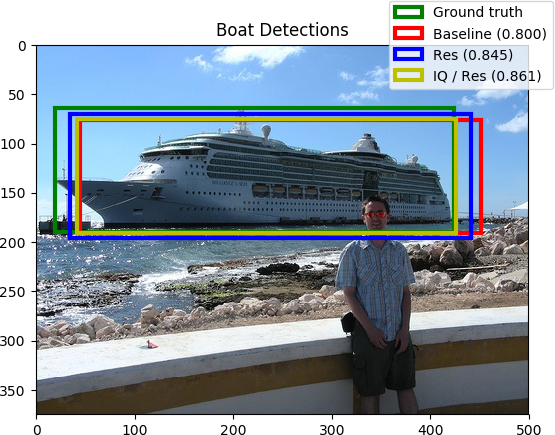
\includegraphics[width=\textwidth]{Figs/Results/000069res.png}
        \caption{}\label{fig:}
    \end{subfigure}
    \begin{subfigure}[b]{0.45\textwidth}
        \center
        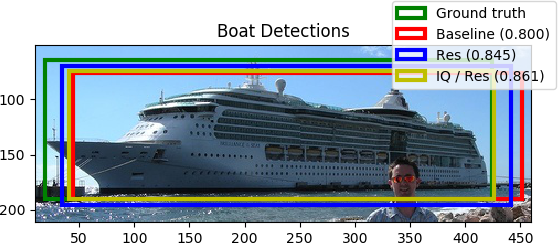
\includegraphics[width=\textwidth]{Figs/Results/000069reszoom.png}
        \caption{}\label{fig:}
    \end{subfigure}
    \caption{Detections for the boat class from an image in the 2007 test set. Shown are the bounding boxes for the ground truth annotation, baseline, Resolution$_{base}$ (Res) and Image Quality$_{WAvg}$ / Resolution$_{Avgbase}$ (IQ / Res). The \gls{iou} between the ground truth and bounding box is shown in parentheses for each method.}
    \label{fig:boatres}
\end{figure} 

\figref{trainres} is an example of a relatively small object in an image. In this instance the best fitting detection is from the Resolution$_{base}$ ensemble with an \gls{iou} of 0.825. An increase of 0.071 compared to the detection with the baseline model. The Image Quality$_{WAvg}$ / Resolution$_{Avgbase}$ also has a better fitting detection with an \gls{iou} of 0.803. The improvement for both ensembles seem to be towards to top of the train  where both bounding boxes fit the ground truth better than the baseline detection.
Again, both models had significant improvements for the train class compared to the baseline model.

\begin{figure}[H]
    \centering
    \begin{subfigure}[b]{0.45\textwidth}
        \center
        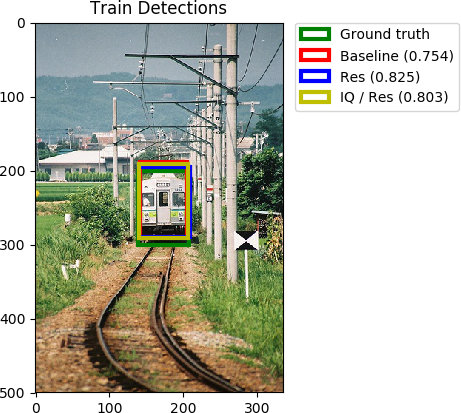
\includegraphics[width=\textwidth]{Figs/Results/000002_res.png}
        \caption{}\label{fig:}
    \end{subfigure}
    \begin{subfigure}[b]{0.45\textwidth}
        \center
        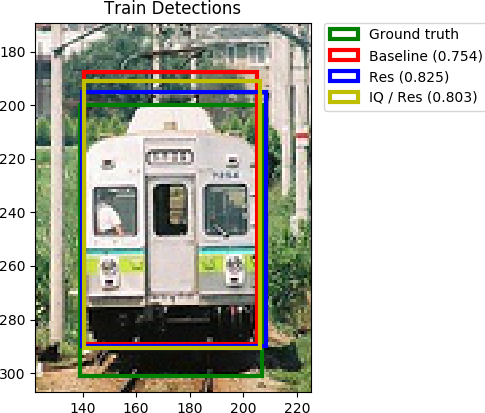
\includegraphics[width=\textwidth]{Figs/Results/000002_reszoom.png}
        \caption{}\label{fig:}
    \end{subfigure}
    \caption{Detections for the train class from an image in the 2007 test set. Shown are the bounding boxes for the ground truth annotation, baseline, Resolution$_{base}$ (Res) and Image Quality$_{WAvg}$ / Resolution$_{Avgbase}$ (IQ / Res). The \gls{iou} between the ground truth and bounding box is shown in parentheses for each method.}
    \label{fig:trainres}
\end{figure} 





